\documentclass[../../thesis.tex]{subfiles}

\graphicspath{{Figures/}}

\begin{document}


\ifSubfilesClassLoaded{
    \tableofcontents
}{}

\chapter{Standard Model of Cosmology} \label{chap:cosmo}
\minitoc

\section*{Introduction}

Cosmology can be described as the science of the Universe, dedicated to understanding its formation and evolution. Within the history of science and physics, cosmology holds a unique position: it is one of the few fields where we cannot replicate phenomena to directly test our theories. We have access to only one Universe, cannot reproduce its mechanisms, and cannot observe all of its information.
This thesis aims to contribute to our understanding of the Universe’s earliest moments. The first chapter provides a structured overview of the Standard Model of Cosmology, called \(\Lambda\)CDM, guiding the reader from its foundational concepts to its current limitations. The chapter is organized into five sections. The first introduces the essential elements of the model, while the second presents the fundamental tools and methods of cosmology. The third section develops the mathematical framework that underpins the model, followed by a discussion of the Universe’s history in the fourth section. Finally, the fifth section highlights the open questions and challenges that continue to drive modern cosmological research.


\rmk{ajouter que je me suis beaucoup inspiré de Dodelson-Schmidt ?}

\section{Evolution of \texorpdfstring{$\Lambda$CDM}{LambdaCDM} Universe}

\rmk{Pas sûr sur ce chapitre... Je voulais faire une sorte d'introduction vulgarisée mais c'est relativement difficile + peut-être pas utile...}

\subsection{Overview - History of the Universe}

\subsection{Hubble Diagram}

\subsection{Big Bang Nucleosynthesis}  

\subsection{Cosmic Microwave Background}

\subsection{Structure of the late Universe}

\subsection{\(\Lambda\)CDM model}

\section{The expanding Universe}

The fundamental milestone of Modern Cosmology was the discovery of its expansion, observed independently by Lema\^itre in 1927~\cite{lemaitre1927} and Hubble in 1929~\cite{hubble1929}. These results changed fundamentally the understanding of the Universe at that time, which was seen as immutable and eternal. This section focuses on the mathematical description of this expansion, and its implication on the Universe.

\subsection{Expansion} \label{subsection:expansion}

The expansion of the Universe was proven by observing the velocity of galaxies around us. Lema\^itre and Hubble measured that the farther the galaxies were from us, the faster they moved away, involving an acceleration of the expansion of the universe. This expansion is characterised by the \emph{scale factor a}. This factor is changing with expansion speed, but is fixed to 1 today by convention. As the expansion is accelerating, this factor was smaller in the past than it is today. It means that the physical distance between two immovable objects will increase proportionally to the scale factor with time, as shown in Figure~\ref{fig:illustration_comoving_distances}. 

\begin{figure}[!htbp]
    \centering
    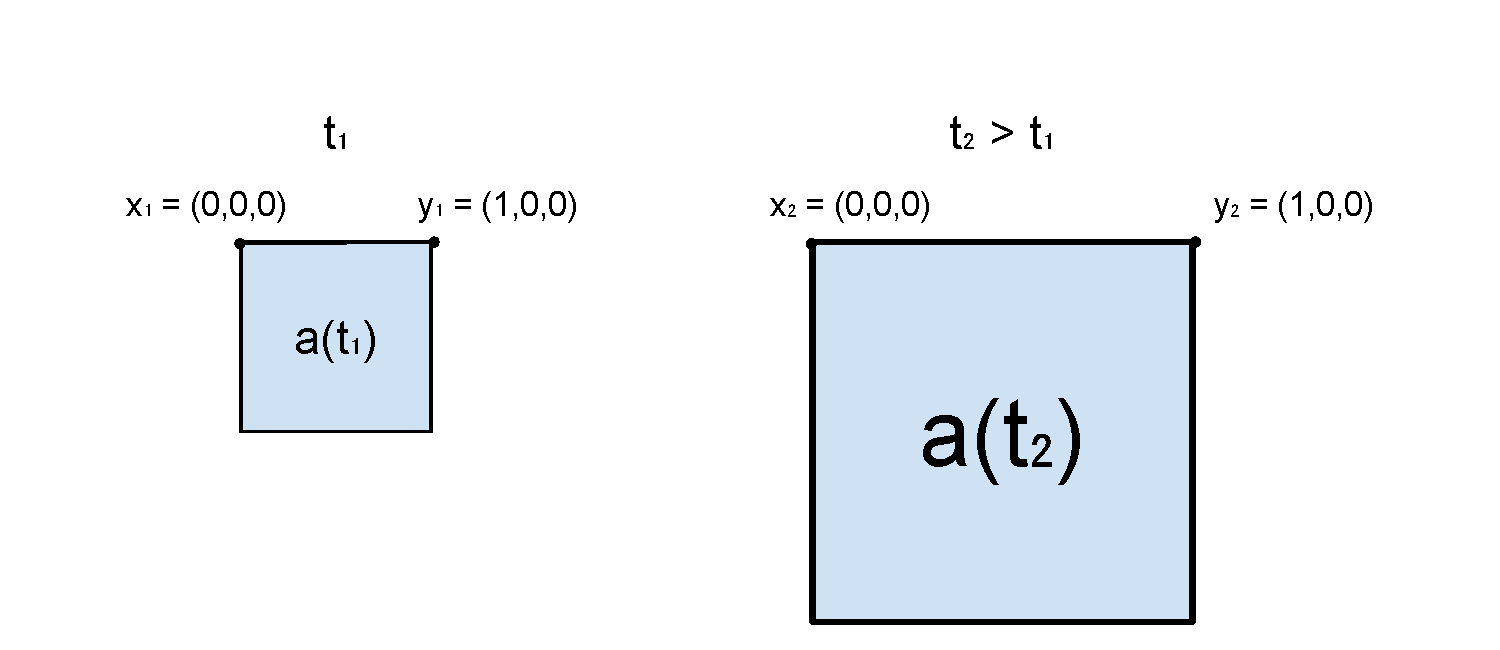
\includegraphics[width=1\linewidth]{illustration_comoving_distances.pdf}
    \caption{Illustration showing the difference between comoving and physical distances. At a time $t_1$, two points $x_1$ and $y_1$ are separated by a distance 1. After some time, at $t_2$, the Universes expanded: the scale factor increased and the physical distance between x and y is larger proportionally to the scale factor. But, the in comoving coordinates, the distance between $x_2$ and $y_2$ is still 1.}
    \label{fig:illustration_comoving_distances}
\end{figure}

A practical example of this phenomenon is the \emph{redshift z}: because the Universe is expanding, the wavelength of a photon is broadened during is travel according to the Doppler effect~\cite{doppler1842}, meaning that this photon is seen as more red. This stretch is proportional to the scale factor, and can be defined as : 

\begin{equation}
    1 + z \equiv \frac{\lambda_{obs}}{\lambda_{emit}} \equiv \frac{a_{obs}}{a_{emit}} = \frac{1}{a_{emit}}
\end{equation}

This property is used to compute velocity of astrophysical objects from us, by measuring the shift of known photon's wavelength like the emission lines from Hydrogen spectrum. If they move away from us, we will see a redshift in the emission lines, and if they come closer to us, we will see a blueshift. In 1929, Edwin Hubble measured velocities for various objects and plotted them with respect to their distance to us~\cite{hubble1929}, as shown in Figure~\ref{fig:hubble_diagram}. In this diagram, we can see that all objects is moving away from us, meaning that the universe is indeed expanding. Furthermore, because the velocity increases with the distance of the objects, it means that the expansion is also accelerating.

\begin{figure}[!htbp]
    \centering
    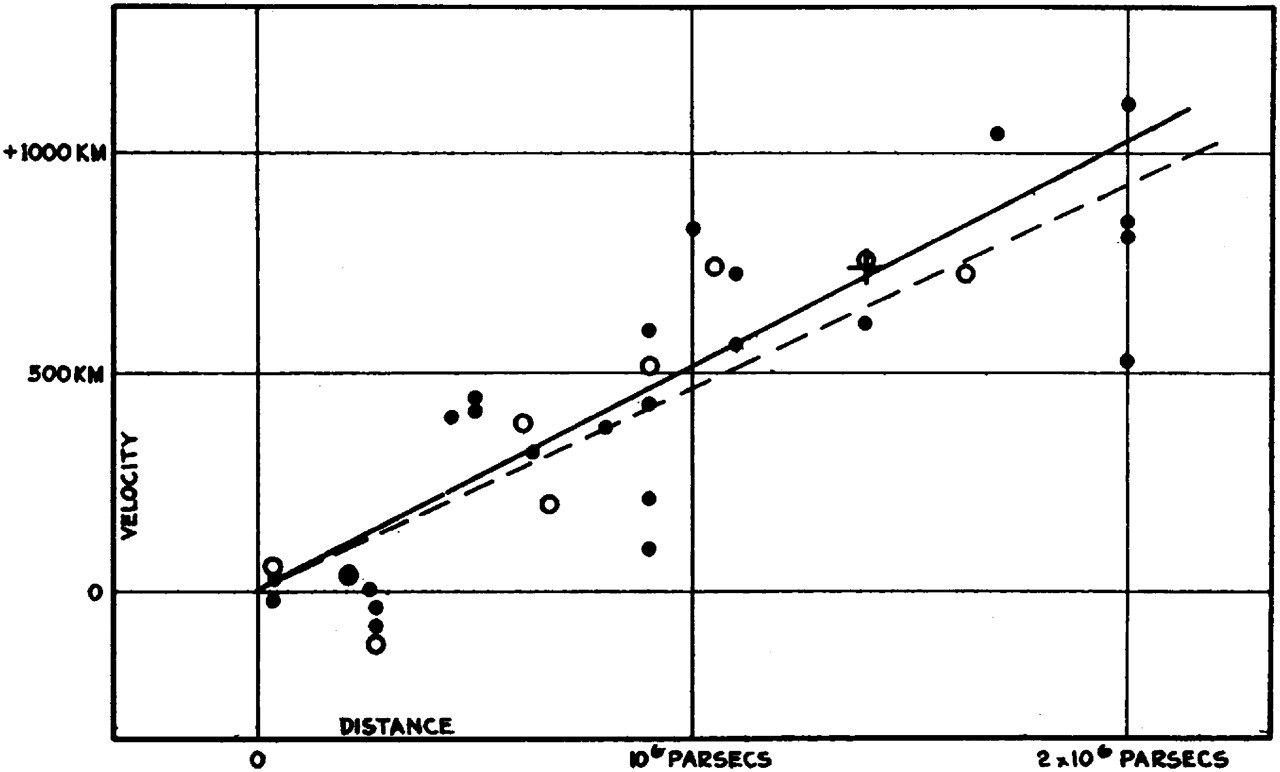
\includegraphics[width=1\linewidth]{hubble_diagram.jpeg}
    \caption{Historical velocity-distance diagram from Edwin Hubble~\cite{hubble1929}. It shows the relative velocity of objects from us against their distance. It shows that furthest the objects are, the quicker they move away from us.}
    \label{fig:hubble_diagram}
\end{figure}


\subsection{Space-time metric}

Additionally to its expansion, the universe is characterised by its geometry. Indeed, it can be Euclidean (flat universe), positively curved (close universe) or negatively curved (open universe). As formulated by General Relativity\cite{generalrelativity1915}, geometry and energy are linked. Therefore, we can extract the universe's geometry from its energy density by comparing it with the energy density needed by the universe to be flat, called \emph{critical density}. If the measured density is smaller than the critical density, the universe is open, if higher, the universe is closed, if equal, the universe if flat. The last situation seems very unlikely, but latest measurement~\cite{planck2018VI} shows that it is indeed the case. This result will be further discussed in the Chapter~\ref{chap:inflation}.

As formulated in Einstein's Special Relativity~\cite{einstein1905}, the metric of an Euclidean space is the Minkowski metric : $g_{\mu\nu} = \eta_{\mu\nu}$, where : 

\begin{equation}
    \eta_{\mu\nu} =
    \begin{pmatrix}
        -1                & 0                 & 0                 & 0     \\
        0                 & 1                 & 0                 & 0     \\
        0                 & 0                 & 1                 & 0     \\
        0                 & 0                 & 0                 & 1     \\
    \end{pmatrix}
\end{equation}

Then, space-time intervals in a flat space are given by : $ds^2 = -c^2dt^2 + dx^2$. 

Hence, we introduce the \emph{scale factor} $a$, which serves as the proportionality factor describing the growth of distances between two points at different times in the expanding Universe. It affects only the spatial part and is time-dependent. The natural metric for a flat expanding universe is then : 

\begin{equation}
    \eta_{\mu\nu} =
    \begin{pmatrix}
        -1                & 0                 & 0                 & 0       \\
        0                 & a^2               & 0                 & 0       \\
        0                 & 0                 & a^2               & 0       \\
        0                 & 0                 & 0                 & a^2     \\
    \end{pmatrix}
\end{equation}

This metric is called the Friedmann-Lema\^itre-Robertson-Walker (FLRW) metric~\cite{friedmann1922}~\cite{lemaitre1927}~\cite{robertson1935}~\cite{walker1936}. This metric can be used to compute space-time distances in a flat expanding universe. One can see that today (at $t = t_0$), the metric becomes the one from Minkowski, as $a(t_0) = 1$.
It is important to notice that this metric is only true for a homogeneous universe. A more general metric would need to account for the local density, meaning the universe inhomogeneities. This will be discussed in the Chapter~\ref{chap:inflation}.

\subsection{Geodesic equation}

\rmk{Je ne pense pas que ça soit nécessaire}

\subsection{Cosmological distances} 

\rmk{Je ne pense pas que ça soit nécessaire}


\section{The fundamental equations of Cosmology}

\subsection{General Relativity}

\subsection{Einstein equation}

\subsection{Friedmann equations}

\subsection{Boltzmann equations}

\section{History of the Universe}

\subsection{Big Bang Nucleosynthesis}

\subsection{Baryons Acoustic Oscillations}

\subsection{Recombination}

\subsection{Reionisation}

\subsection{Large Scale Structure}

\section{Problems of the Standard Model}

\subsection{Horizon Problem}

\subsection{Flatness Problem}

\subsection{Monopole Problem}

\ifSubfilesClassLoaded{
    \addstarredchapter{Bibliography}
    \printbibliography
}{}

\end{document}
